\documentclass{beamer}

% Theme choice:
\usetheme{CambridgeUS}
\usepackage{amsmath}
\usepackage{mathtools}
\providecommand{\pr}[1]{\ensuremath{\Pr\left(#1\right)}}
\providecommand{\cdf}[2]{\ensuremath{\text{F}_{#1}\left(#2\right)}}
\providecommand{\erf}[1]{\ensuremath{\text{erf}(#1)}}
\setbeamertemplate{caption}[numbered]
% Title page details: 
\title{Dimesionality Reduction using PCA, ICA and generalized PCA} 
\author{Lokesh Surana (ES20BTECH11017)\\ Samar Singhai (BM20BTECH11012)}
\date{\today}

\begin{document}

% Title page frame
\begin{frame}
    \titlepage
\end{frame}

% Outline frame
\begin{frame}[allowframebreaks]{Outline}
    \tableofcontents
\end{frame}

\section{Dimensionality reduction}
\begin{frame}{What is dimensionality reduction?}
    \begin{enumerate}
        \item A technique in machine learning and data analysis. It allows us to simplify high-dimensional data sets by identifying the most important features and reducing the number of dimensions.
        \item This can improve the efficiency and accuracy of algorithms, as well as help us gain a better understanding of the underlying patterns and relationships in the data.
        \item \textbf{What are benifits of dimensional reduction?}
    \end{enumerate}
\end{frame}

\begin{frame}{What is dimensionality reduction?}
    \begin{figure}
        \centering
        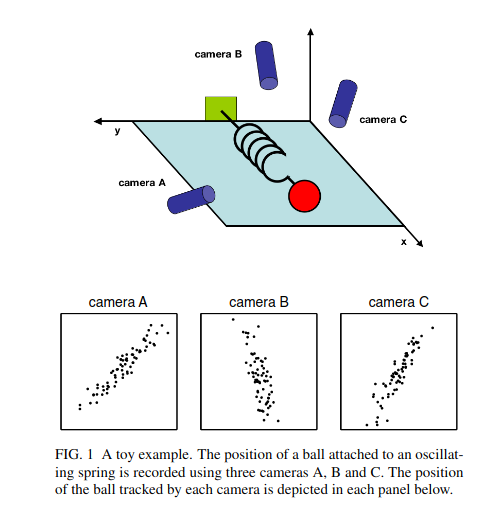
\includegraphics[width=0.6\textwidth]{toy_readings.png}
        \caption{Dimensionality reduction}
        \label{fig:my_label}
    \end{figure}
\end{frame}

\begin{frame}{Why dimensionality reduction is important?}
    \begin{enumerate}
        \item \textbf{Speed up computations:} High-dimensional data requires a lot of computational resources to analyze, and working with such data can be very time-consuming. By reducing the dimensions of the data, we can speed up the computation and make it more efficient.
        \item \textbf{Visualization:} High-dimensional data is difficult to visualize, but by reducing the dimensions of the data, we can plot the data in 2D or 3D and visualize the relationships between different variables.
        \item \textbf{Improves model performance:} In many machine learning tasks, high-dimensional data can lead to overfitting and other problems. By reducing the dimensions of the data, we can improve the performance of our models and reduce the risk of overfitting.
    \end{enumerate}
\end{frame}

\begin{frame}{Signal to Noise Ratio}
    \begin{figure}
        \centering
        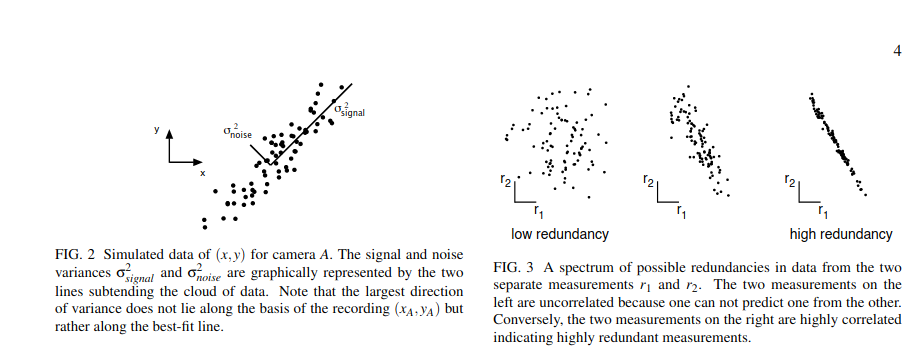
\includegraphics[width=0.8\textwidth]{SNR.png}
        \caption{Signal to Noise Ratio}
        \label{fig:signal_noise_ratio}
    \end{figure}
\end{frame}

\section{Principal Component Analysis}
\subsection{Concept}

\begin{frame}{PCA}
    \begin{enumerate}
        \item The motivation behind Principal Component Analysis (PCA) is to reduce the dimensionality of a dataset while retaining as much of the variation in the data as possible. This is useful when the original dataset has many features or variables, making it difficult to visualize or analyze the data.
        \item By identifying the principal components of the data, linear combinations of the original variables, PCA can represent the data in a lower-dimensional space that still captures the essential patterns of variation in the original data.
        \item PCA can also perform data compression since the principal components can be used to reconstruct the original data with some loss of information.
        \item PCA can be used to remove noise from the data since the principal components correspond to the directions of maximal variance in the data and are, therefore, less likely to be affected by noise.
    \end{enumerate}
\end{frame}

\subsection{Mathematics involved in PCA}
\begin{frame}{Variance}
    \begin{enumerate}
        \item A statistical measure that quantifies the amount of spread or dispersion in a dataset. It measures how far a set of data points are spread out from the mean.
        \item  In PCA, the variance of a dataset is the amount of information or variation contained in that dataset. The first principal component captures the maximum amount of variation in the data. Subsequent principal components capture progressively smaller amounts of variation.
        \item The eigenvalues measure the amount of information or variation in the data captured by each principal component.
        \item The sum of all eigenvalues is equal to the total variance of the data. Therefore, the proportion of variance a principal component explains can be calculated as the ratio of its eigenvalue to the sum of all eigenvalues - "explained variance ratio."

    \end{enumerate}
\end{frame}


\begin{frame}{The covariance matrix}
    \begin{enumerate}
        \item A \textbf{symmetric square matrix} that summarizes the relationships between variables in a dataset.
        \item Covariance matrix is \textbf{positive semi-definite} - all of its eigenvalues are non-negative.
        \item The covariance matrix determine the degree of correlation between the variables in the data set. If the covariance between two variables is positive, the variables tend to move in the same direction. On the other hand, if the covariance is negative, the variables tend to move in opposite directions. If the covariance is zero - no correlation.
        \item In the context of PCA, it is a measure of the variability in the data. The covariance matrix provides information about \textbf{how much the variables in the data set vary from the mean and how they are related?}
    \end{enumerate}
\end{frame}

\begin{frame}{Eigenvectors and eigenvalues and their properties }
    \begin{enumerate}
        \item An eigenvector is a non-zero vector that, when multiplied by a matrix, results in a scalar multiple of the original vector. This scalar multiple is called the eigenvalue.
        \item \textbf{Orthogonality:} Eigenvectors corresponding to distinct eigenvalues are orthogonal to each other, meaning they are perpendicular in n-dimensional space. \textbf{This property is useful for separating different sources of variation in a dataset.}
        \item \textbf{Normalization:} Eigenvectors are typically normalized to have unit length. \textbf{This ensures that the magnitude of the eigenvectors does not affect their contribution to the principal components.}
    \end{enumerate}
\end{frame}

\begin{frame}{Principal Component}
    \begin{enumerate}
        \item This components are new variables that are linear combinations of the original variables.
        \item The first principal component is a linear combination of the original variables that captures the largest variation in the data. The second principal component is a linear combination of the original variables that captures the largest amount of variation that is orthogonal (uncorrelated) to the first principal component, and so on.
        \item By using eigenvectors and eigenvalues of the covariance matrix, principal components are derived. The eigenvectors represent the directions of maximum variance in the data, and the eigenvalues indicate the amount of variance explained by each eigenvector. \
    \end{enumerate}
\end{frame}

\begin{frame}{How eigenvectors and eigenvalues are used to obtain principal components?}
    \begin{enumerate}
        \item \textbf{The first principal component is a linear combination of the original variables that captures the largest amount of variation in the data}, and subsequent principal components capture orthogonal variation in decreasing order of importance.
        \item Compute the covariance matrix of the dataset $\rightarrow$ Calculate the eigenvectors and eigenvalues of the covariance matrix $\rightarrow$ Sort the eigenvectors by their corresponding eigenvalues in descending order $\rightarrow$ Select the top k eigenvectors with the highest eigenvalues to form the principal components $\rightarrow$ Project the original data onto the k principal components to obtain the lower-dimensional representation.
    \end{enumerate}
\end{frame}

\subsection{Pseduo Code}
\begin{frame}{Pseduo Code for PCA}
    \begin{enumerate}
        \item Input: \\
              - X: matrix of size (n, m), where n is the number of samples and m is the number of features\\
              - k: number of principal components to keep
        \item 1. Standardize the data - Calculate the mean of each column of X, subtract it from the corresponding column, and divide by the standard deviation of that column. This produces a standardized version of X with mean 0 and variance 1 for each feature.
        \item 2. Compute the covariance matrix - Calculate the covariance matrix of the standardized data using the formula $cov(X) = \frac{XX^T}{n - 1}$
        \item 3. Compute the eigenvectors and eigenvalues of the covariance matrix: Use an eigendecomposition method, such as the power iteration method or the QR algorithm

    \end{enumerate}
\end{frame}

\begin{frame}{Pseduo Code for PCA}
    \begin{enumerate}
        \item 4. Sort the eigenvectors in decreasing order of eigenvalue: Select the k eigenvectors with the largest eigenvalues, and store them in a matrix V.
        \item 5. Project the data onto the new k-dimensional space: Compute the matrix product X' = X * V, where X' is the new matrix of size (n, k) representing the data projected onto the k-dimensional space defined by the eigenvectors.
        \item output:\\
              - X': matrix of size (n, k) representing the data projected onto the k-dimensional space defined by the eigenvectors.

    \end{enumerate}
\end{frame}

\subsection{Applications}
\begin{frame}{Applications}
    \begin{enumerate}
        \item \textbf{Few of the applications of PCA are:}
        \item In genetics, PCA can be used to identify the most important genes and reduce the dimensions of the data, making it easier to analyze and understand the relationships between different genes.
        \item In finance, PCA can be used to identify the most important trends and patterns in stock prices and reduce the dimensions of the data, making it easier to analyze and predict future trends.
        \item 
    \end{enumerate}
\end{frame}

\subsection{Limitations}
\begin{frame}{Limitations of PCA}
    \begin{enumerate}
        \item PCA assumes that the relationship between variables is linear. This means that PCA may not be appropriate for datasets that contain non-linear relationships between variables, such as those that exhibit complex or nonlinear patterns.
        \item Assumes that the principal components are orthogonal, meaning they are uncorrelated. This assumption may not hold in some cases, such as when dependencies or interactions between variables violate the orthogonality assumption.
        \item PCA can also be sensitive to outliers in the data. Outliers can skew the results of PCA, as they can disproportionately influence the principal components.
    \end{enumerate}
\end{frame}

\begin{frame}{Other techniques?}
    \begin{enumerate}
        \item Other dimensionality reduction techniques include Independent Component Analysis (ICA), which aims to identify underlying independent sources of variation in the data, and Kernel PCA, which extends PCA to non-linearly separable data by projecting the data onto a higher-dimensional space. These techniques can be useful when dealing with complex or non-linear data sets.
    \end{enumerate}
\end{frame}

\section{Independent Component Analysis (ICA)}
\subsection{Concept}
\begin{frame}{Concept}
    \begin{enumerate}
        \item Independent Component Analysis (ICA) is a dimensionality reduction technique that is motivated by the desire to separate a multivariate signal into its independent components or sources. In many real-world applications, such as speech processing or image analysis, signals are often mixed together, making it difficult to separate individual sources.
        \item  ICA aims to overcome this challenge by identifying the underlying sources and their corresponding mixing coefficients, even if the signals are mixed in an unknown and nonlinear way.
        \item ICA has various applications in signal processing, such as speech separation, image processing, and data compression. By separating the independent sources, ICA can reveal hidden information and improve the quality of the processed signals
    \end{enumerate}
\end{frame}

\subsection{How ICA works?}
\begin{frame}{How ICA works?}
    \begin{enumerate}
        \item ICA is based on the following assumptions\\
              The main assumptions of ICA are statistical independence and non-Gaussianity of the sources. ICA uses a maximum likelihood approach to estimate the independent components.
        \item Let X be a random vector of observed signals, and A be an unknown matrix representing the mixing process that transforms the original sources S into the observed signals X, such that X = AS. The goal of ICA is to estimate the matrix A and the independent sources S, given only the observed signals X.
        \item The first assumption of ICA is that the sources S are statistically independent. This means that the joint probability distribution of the sources can be factorized as P(S) = $\pi P(S_i)$, where Si is the i-th component of the source vector S. In other words, the sources are not correlated with each other and contain different information.

    \end{enumerate}
\end{frame}

\begin{frame}{How ICA works?}
    \begin{enumerate}
        \item The second assumption of ICA is that the sources S are non-Gaussian. This is because Gaussian sources can be linearly mixed to form a Gaussian distribution, making it impossible to recover the original sources. Non-Gaussian sources, on the other hand, retain their independence even when mixed, making it possible to separate them.
        \item The maximum likelihood estimation approach used in ICA aims to estimate the independent components by maximizing the likelihood function of the observed signals X. The likelihood function is defined as the joint probability density function of the observed signals, given the mixing matrix A and the independent sources S, i.e., L(A,S|X) = P(X|A,S). Using the assumptions of statistical independence and non-Gaussianity, the likelihood function can be maximized using methods such as gradient ascent or fixed-point iteration.
    \end{enumerate}
\end{frame}

\subsection{Pseduo Code}
\begin{frame}{Pseduo Code}
    \begin{enumerate}
        \item Input: \newline
        - X: Observed signals (matrix of size n X m) \newline
        - n-components: Number of independent components to estimate
        \item 1.Center the observed signals by subtracting the mean of each column of X from the corresponding column.
        \item 2.Whiten the observed signals by applying a whitening transform to X-centered. Whitening the data transforms the data into a new space where the covariance matrix is diagonal, and each feature's variance equals one. This makes the estimation of the independent components easier.
        \item 3.Initializing the unmixing matrix randomly (starts the estimation process).
    \end{enumerate}
\end{frame}


\begin{frame}{Pseduo Code}
    \begin{enumerate}
        \item 4.The main estimation loop updates the unmixing matrix A by performing gradient ascent on the likelihood function. The nonlinearity function is applied to the estimated sources to make the problem non-Gaussian. The step size controls the learning rate of the algorithm, and the orthonormalization step ensures that the unmixing matrix is orthonormal.
        \item 5.The estimated independent sources are computed by applying the inverse transformation of whitening and centering to the unmixing matrix.
        \item 6.The estimated independent sources are returned as output.
        \item Output: \newline
        S: Estimated independent sources (matrix of size n x n-components)
    \end{enumerate}
\end{frame}

\subsection{Applications}
\begin{frame}{Applications}
    \begin{enumerate}
        \item Speech Separation: ICA can be used to separate different speakers' voices from a single audio recording. The assumption of statistical independence allows ICA to separate the sources by identifying the independent components in the mixed signal. The non-Gaussianity assumption helps ICA to identify the non-Gaussian speech components, which can be used to separate the sources.
        \item EEG Analysis: EEG signals are generated by the electrical activity of the brain, and ICA can be used to separate the sources of these signals. The statistical independence assumption allows ICA to identify the independent components of the EEG signals, such as alpha, beta, and gamma waves. The non-Gaussianity assumption helps to identify the non-Gaussian components, which may represent artifact or noise components.
    \end{enumerate}
\end{frame}

\subsection{Limitations}
\begin{frame}{Limitations of ICA}
    \begin{enumerate}
        \item \textbf{Non-Gaussianity assumption: }ICA assumes that the independent components are non-Gaussian, which may not hold in all cases. Some independent components may be Gaussian, making separating the sources difficult or impossible. 
        \item ICA assumes that the observed signals are linear mixtures of the independent components. If the mixing process is nonlinear, ICA may not be able to separate the sources. Moreover, ICA assumes that the mixing process is instantaneous and does not take into account any delays or temporal dependencies between the sources.
        \item ICA is sensitive to the initial conditions of the estimation process. Depending on the initial unmixing matrix, the algorithm may converge to different solutions, which can lead to different estimates of the independent components. So different initializations have to be tried and compare the results to ensure the robustness of the estimates.
    \end{enumerate}
\end{frame}

\begin{frame}{Limitations}
    \begin{enumerate}
        \item ICA requires the specification of the number of independent components to estimate, which can be difficult to determine in practice. If the number of estimated components is too high, some components may be redundant or contain noise. Some important sources may be missed if the number of estimated components is too low. So, \textbf{the choice of the number of independent components} may require trial and error or prior knowledge about the problem.
        \item ICA can be \textbf{computationally expensive}, especially for large datasets or high-dimensional signals. The whitening and unmixing steps require matrix decompositions and multiplications, which can be time-consuming. Moreover, the optimization process may require a large number of iterations to converge, which can increase the computational cost.
    \end{enumerate}
\end{frame}

\section{Generalized PCA}
\subsection{Concept}
\begin{frame}{What and why?}
    \begin{enumerate}
        \item The motivation behind generalized PCA is to address the limitations of traditional PCA methods, which assume that the data follows a Gaussian distribution and that the relationships between variables are linear.
        \item Generalized PCA aims to extend PCA to handle non-Gaussian distributions and non-linear relationships between variables. This can improve the accuracy and usefulness of PCA in various applications, such as image and signal processing, where non-linear and non-Gaussian relationships are common. By incorporating non-linear relationships and non-Gaussian distributions, generalized PCA can capture more complex and meaningful patterns in the data.
    \end{enumerate}
\end{frame}

\subsection{How Generalized PCA works?}
\begin{frame}{How Generalized PCA works?}
    \begin{enumerate}
        \item One approach is to use the kernel trick, which allows us to perform non-linear transformations of the data without explicitly computing them. Specifically, the kernel trick involves mapping the original data points into a higher-dimensional feature space using a non-linear function and then computing the principal components in this feature space.
        \item Kernel PCA is a specific instance of the kernel trick, where the principal components are computed using the kernel matrix instead of the original data matrix. The kernel matrix is computed by applying the kernel function to all pairs of data points and can be efficiently computed using matrix operations.
        \item Another approach is to use other non-linear techniques, such as manifold learning methods, which aim to discover the underlying low-dimensional structure of the data by preserving the local geometry of the data. Examples of manifold learning methods include Isomap, Locally Linear Embedding (LLE), and t-Distributed Stochastic Neighbor Embedding (t-SNE).
    \end{enumerate}
\end{frame}

\subsection{Pseduo Code}
\begin{frame}{Pseduo Code}
    The generalized PCA method is implemented through the following steps:
    \begin{enumerate}
    \item Solve the quasi covariance matrix. \newline
    $R^\prime = \Sigma B(x_i - \bar{x_i})(x_i - \bar{x_i})^\top B^\top$
    \item Find the eigenvalues of the quasi covariance matrix and arrange them in descending order.
    \item Normalize the eigenvectors.
    \item Select the first few feature vectors for dimensionality reduction.
    \item Calculate the dimensionality reduction results.
    \end{enumerate}
\end{frame}

\begin{frame}[allowframebreaks]{Pseduo Code for Kernel PCA}
    Input: Data matrix X, kernel function K, \newline number of principal components k
    \begin{enumerate}
    \item Compute the kernel matrix K-prime, which is a matrix that captures the similarity between pairs of data points in X using a kernel function K.
    \item Center the kernel matrix K-prime by subtracting the mean of each row and column. This is done to ensure that the principal components are computed with respect to the covariance matrix of the data.
    \item Compute the eigendecomposition of the centered kernel matrix K-centered to obtain the eigenvalues and eigenvectors of the covariance matrix of the data.
    \item Select the top k eigenvectors corresponding to the largest eigenvalues, and normalize them to have unit length. These eigenvectors define the k-dimensional subspace that captures the most variance in the data.
    \item Project the original data matrix X onto the k-dimensional subspace by computing the dot product between each data point and the k eigenvectors. This results in a k-dimensional representation of the data that captures the most important information.
    \item The output of the algorithm is the k-dimensional representation of the data (Z), the eigenvalues (eigvals), and the eigenvectors (eigvecs) of the covariance matrix.
    \end{enumerate}
\end{frame}

\subsection{Applications}
\begin{frame}{Applications}
    \begin{enumerate}
        \item \textbf{Image Processing:} Generalized PCA can be used for image compression and feature extraction. For instance, in face recognition, a kernel PCA can be applied to the face images to extract the principal components that capture the variations in the face images. These principal components can then represent the faces in a lower dimensional space, reducing the computational complexity of face recognition algorithms.
       \item \textbf{Bioinformatics:} Generalized PCA can be used to analyze gene expression data and identify the genes most correlated with a particular disease or condition. For example, kernel PCA can be used in cancer research to identify the genes that are differentially expressed between cancerous and healthy tissues. These genes can then be used to develop diagnostic tests or therapeutic targets.
    \end{enumerate}
\end{frame}

\subsection{Limitations}
\begin{frame}[allowframebreaks]{Limitations of Generalized PCA}
    \begin{enumerate}
        \item The \textbf{choice of kernel function} greatly affects the results of generalized PCA. Different kernels have different properties and may be more appropriate for certain types of data. Therefore, choosing the right kernel is crucial for obtaining accurate and meaningful results. However, there is no universally optimal kernel for all types of data, and the choice of kernel often requires prior knowledge or experimentation.
        \item \textbf{Difficulty interpreting non-linear relationships:} Generalized PCA can capture non-linear relationships between variables, a major advantage over traditional PCA. However, non-linear relationships can be difficult to interpret and may not have a simple intuitive explanation. This can make it challenging to gain insights and draw meaningful conclusions from the results of generalized PCA.
        \item Generalized PCA involves computing the kernel matrix, which can be \textbf{computationally expensive} for large datasets. In addition, computing the eigendecomposition of the kernel matrix can also be time-consuming. 
        \item \textbf{Overfitting:} Generalized PCA can overfit the data if the number of principal components is too high. This can result in the model capturing noise and other irrelevant information in the data, which can lead to poor performance on new data. Regularization techniques such as ridge regression can be used to address this issue.
    \end{enumerate}
\end{frame}

\end{document}